\documentclass{article}

% Language setting
% Replace `english' with e.g. `spanish' to change the document language
%\usepackage[english]{babel}
\usepackage[UTF8]{ctex}
\usepackage{setspace}
\usepackage{listings}
\usepackage{xcolor}
\usepackage{tikz}
\usepackage[colorlinks,linkcolor=blue]{hyperref}
\usepackage{float}

\lstset{
  backgroundcolor=\color{white},
  basicstyle=\ttfamily\footnotesize,
  breakatwhitespace=false,
  breaklines=true,
  captionpos=b,
  commentstyle=\color{mygreen},
  deletekeywords={...},
  escapeinside={\%*}{*)},
  frame=single,
  keepspaces=true,
  keywordstyle=\color{blue},
  language=Python,
  morekeywords={*,...},
  numbers=left,
  numbersep=5pt,
  numberstyle=\tiny\color{mygray},
  rulecolor=\color{black},
  showspaces=false,
  showstringspaces=false,
  showtabs=false,
  stepnumber=2,
  stringstyle=\color{mymauve},
  tabsize=2,
  title=\lstname
}
% Set page size and margins
% Replace `letterpaper' with `a4paper' for UK/EU standard size
\usepackage[letterpaper,top=2cm,bottom=2cm,left=3cm,right=3cm,marginparwidth=1.75cm]{geometry}

% Useful packages
\usepackage{amsmath}
\usepackage{graphicx}
\usepackage[colorlinks=true, allcolors=blue]{hyperref}

\title{当代人工智能实验报告2}
\author{温兆和 10205501432}

\begin{document}
\maketitle

\section{实验目的}
这一次的实验是用A*算法解决两个问题。

\section{实验环境}
PyCharm 2022.1

Python 3.10

\textbf{需要安装的工具包有:}
\begin{spacing}{0.5}
\begin{itemize}
\item \lstinline|queue|
\item \lstinline|sys|
\end{itemize}
\end{spacing}
如果有哪个工具包(假设叫\lstinline|X|)需要安装,就同时按\lstinline|Win|+\lstinline|R|,选择\lstinline|cmd|,在Window shell里面执行\lstinline|pip install X|即可,或者也可以执行\lstinline|pip install -r requirements.txt|来安装这些包。

\section{问题一:冰雪魔⽅的冰霜之道}

\subsection{问题内容}
在遥远的冰雪王国中,存在⼀个由$9$个神秘冰块组成的魔法魔⽅。在这个魔法魔⽅中,有$8$块冰雪魔块,每块都雕刻有$1$-$8$中的⼀个数字(每个数字都是独特的)。魔⽅上还有⼀个没有雕刻数字的空冰块,⽤$0$表示。你可以滑动与空冰块相邻的冰块来改变魔块的位置。传说,当冰雪魔块按照⼀个特定的顺序排列(设定为$1$ $3$ $5$ $7$ $0$ $2$ $6$ $8$ $4$)时,魔法魔⽅将会显出通往⼀个隐秘冰宫的冰霜之道。现在,你站在这个神秘的魔⽅前,试图通过最少的滑动步骤将冰雪魔块排列成⽬标顺序。为了揭开这⼀秘密,你决定设计⼀个程序来从初始状态成功找到冰霜之道。


\subsection{解决思路}
这个问题本质上是这样的:在一个$3*3$的九宫格中放着八个数字,九宫格中还有一个空位。给定初始状态后,可以把空位周边的数字移到空位上,每移动一次代价为$1$,最终要通过A*算法来找到代价最小的移动步骤,让九宫格中的数字按照特定顺序排列,并输出最小移动代价。

在使用A*算法解决问题之前,我们需要先定义每移动一步的代价和启发式函数。在这个问题里,我们把每移动一次数字的代价定义为$1$。启发式函数是从状态到数字的映射,代表从这个状态到目标状态的代价的估计值。为了保证A*算法一定能够得到最优解,启发式函数必须满足一定的条件。具体来说,在树搜索中,启发式函数必须admissible(可容许),也就是说它不能过高地估计从当前状态到目标状态的代价;在图搜索中,启发式函数还必须具有consistency(一致性),也就是说,假设一个状态有后继状态,那么这个状态到目标节点的估计代价必须小于从这个节点到它某一个子节点的实际代价与那个子节点到目标状态的估计代价。一致性包含可容许性。一般来说,对实际的移动过程进行一定的松弛就能得到admissible的启发式函数。所以,在这个问题中,我们可以把“不在位的数码个数”作为启发式函数的值。
\begin{lstlisting}
def heuristic(state):
    sum = 0
    for i in range(9):
        if state[i] != 0:
            if state[i] != goal_state[i]:
                sum+=1
    return sum
\end{lstlisting}
比如,如果当前状态是
\begin{center}
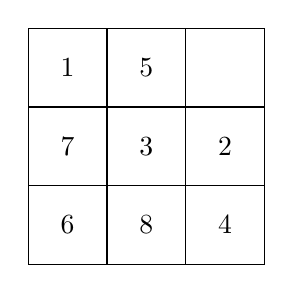
\begin{tikzpicture}
  \draw (0,0) rectangle (3,3);
  
  \draw (1,0) -- (1,3);
  \draw (2,0) -- (2,3);
  \draw (0,1) -- (3,1);
  \draw (0,2) -- (3,2);
  \node at (0.5, 2.5) {1};
  \node at (1.5, 2.5) {5};
  \node at (2.5, 2.5) { };
  \node at (0.5, 1.5) {7};
  \node at (1.5, 1.5) {3};
  \node at (2.5, 1.5) {2};
  \node at (0.5, 0.5) {6};
  \node at (1.5, 0.5) {8};
  \node at (2.5, 0.5) {4};
\end{tikzpicture}
\end{center}
容易看出总共有$5$、$3$这两个数字的位置与目标状态不同。所以,这个状态的启发式函数的值为$2$。王万良的《人工智能导论》中说到,这个启发式函数是admissible的\textsuperscript{~\hyperref[ref1]{[1]}}。

有了启发式函数、每移动一步的代价、初始状态和目标状态,我们就可以用A*算法解决这个问题了。首先,A*算法需要不断地寻找当前节点的子节点中“已经付出的代价”和“到达目标状态还要付出的代价的估计值”之和(以下简称“某状态的$f(n)$值”)最小的那一个,所以用“优先级队列”这个数据结构来实现这个算法最合适。Python中已经有现成的优先级队列,可以直接使用。
\begin{lstlisting}
from queue import PriorityQueue
open_list = PriorityQueue()
\end{lstlisting}

在算法开始运行之前,我们首先要将初始状态压入优先级队列中。值得注意的是,每一个状态需要用一个元组来表示,元组中应含有该状态的$f(n)$值、该状态下数字的顺序和该状态启发式函数的值。其中,$f(n)$值必须放在元组的第一位,这样优先级队列在弹出时就以这个量作为弹出的依据。此外,为了避免不必要的重复运算,我们不会重新走到已经走过的状态下,所以必须维护一个集合来存放已经经历过的状态。
\begin{lstlisting}
open_list.put((heuristic(initial_state), initial_state, 0))
closed_set = set()
while not open_list.empty():
    ……
    if current_state in closed_set:
        continue
\end{lstlisting}

在进入\lstinline|while|循环后,我们不断地执行\lstinline|open_list.get()|函数,从优先级队列中获取$f(n)$值最小的状态,在确保没有经历过这个状态的前提下将当前状态加入集合\lstinline|closed_set|,并计算当前状态所有子节点的启发式函数值和$f(n)$值,将所有子节点压入优先级队列。
\begin{lstlisting}
closed_set.add(current_state)
for direction in ['left', 'right', 'up', 'down']:
    new_state = move(current_state, direction)
    open_list.put((heuristic(new_state) + g + 1, new_state, g + 1))
\end{lstlisting}

退出\lstinline|while|循环无非就是两种情况:要么是到达了目标状态,直接停止循环并返回最小移动次数,要么是优先级队列被清空还没有到达目标状态,返回“无法到达目标状态”的信息。
\begin{lstlisting}
steps = astar(initial_state)
if steps >= 0:
    print(steps)
else:
    print("无解")
\end{lstlisting}

我们把实验手册中提供的例子作为输入运行这个算法,得到了正确的输出。
\begin{figure}[H]
    \centering
    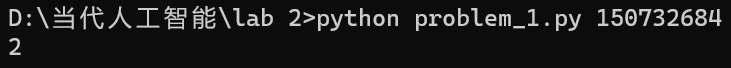
\includegraphics[width=0.5\linewidth]{image7.png}
    %\caption{Enter Caption}
    \label{fig:enter-label}
\end{figure}

\subsection{测试结果}
我们在Windows的命令行中进入项目路径,用\lstinline|python problem_1.py {输入值}|命令来运行这个程序。将实验手册中的五个测试用例分别作为输入来运行我们刚刚实现的算法,结果如下图所示:
\begin{figure}[H]
    \centering
    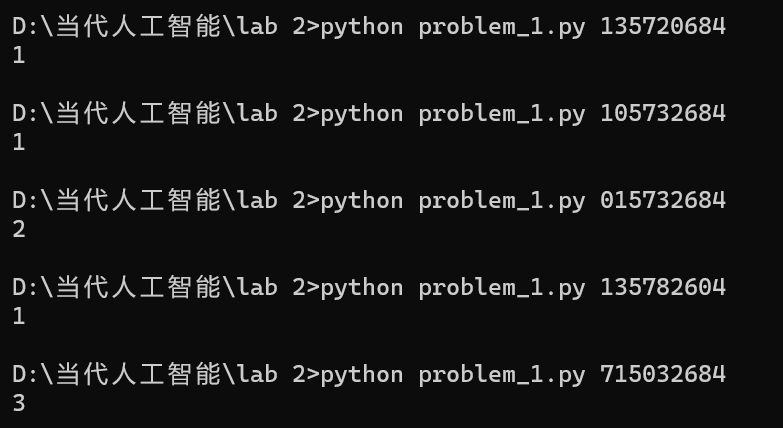
\includegraphics[width=0.5\linewidth]{image1.png}
    %\caption{Enter Caption}
    \label{fig:enter-label}
\end{figure}

\section{问题二:杰克的⾦字塔探险}
\subsection{问题内容}
在⼀个神秘的王国⾥,有⼀个名叫杰克的冒险家,他对宝藏情有独钟。传说在那⽚⼴袤的⼟地上,有⼀座名叫⾦字塔的奇迹,隐藏着⽆尽的财富。杰克决定寻找这座⾦字塔,挖掘隐藏在其中的宝藏。⾦字塔共有$N$个神秘的房间,其中$1$号房间位于塔顶,$N$号房间位于塔底。在这些房间之间,有先知们预先设计好的$M$条秘密通道。这些房间按照它们所在的楼层顺序进⾏了编号。杰克想从塔顶房间⼀直探险到塔底,带⾛尽可能多的宝藏。
然⽽,杰克对寻宝路线有着特别的要求:
%\begin{spacing}{0.3}
\begin{enumerate}
\item 他希望⾛尽可能短的路径,但为了让探险更有趣和挑战性,他想尝试$K$条不同的较短路径。
\item 他希望在探险过程中尽量节省体⼒,所以在选择通道时,他总是从所在楼层的⾼处到低处。
\end{enumerate}
%\end{spacing}

现在问题来了,给你⼀份⾦字塔内房间之间通道的列表,每条通道⽤($X_i$,$Y_i$,$D_i$)表⽰,表⽰房间$X_i$和房间$Y_i$之间有⼀条长度为$D_i$的下⾏通道。你需要计算出杰克可以选择的$K$条最短路径的长度,以便了解他在探险过程中的消耗程度。

\subsection{解决思路}
这个问题本质上和课上讲的罗马尼亚旅行问题差别不大,无非就是输入一个有向加权图,指定初始节点和目标节点,要求找出代价最小的几条路径。最主要的区别就是课上讲的例子只要输出一条最短路径,而这个问题需要输出前$K$短的路径。课上讲到当我们用A*算法解决问题时,要从优先级队列中弹出一次目标状态才能停止,那在这个问题中我们就需要到弹出$K$次目标状态或者找不到更多的路径时才能停止迭代。

在这个问题中,从一个状态转移到另一个状态的代价已经给定,我们只需要自己定义一个启发式函数。在这个问题中,"$1$号房位于塔顶,$N$号房位于塔底,房间按照楼层顺序编号",而且杰克是要从塔顶的$1$号房一直走到塔底的$N$号房的。如果说要对实际的代价进行一些松弛,我们自然会认为两个房间的编号差越大,它们之间间隔的楼层数越多,从其中一个房间走到另一个房间的代价也就越大。所以,某个状态(也就是所处房间)启发式函数的值就是目标房间($N$号房)与这个房间的编号之差。此外,为了保证这个启发式函数具有consistency,我们还需要对这个差值进行一些调整,让它的值始终不超过$1$。如果一个启发式函数具有consistency,那么对任意一个状态$n$和它的任意子节点$n^*$,都有
$$h(n)\leq g(n,n^*)+h(n^*)$$
其中$h(·)$是启发式函数,$g(n,n^*)$指的是从状态$n$转移到它的子节点$n^*$的实际代价。由于在实验手册的所有测试用例中从一个状态转移到其子节点的实际代价都至少为$1$,所以$$g(n,n^*)\geq 1, {\forall}n,n^*$$
又因为
$$h(n)\leq 1, {\forall}n$$
所以必然有
$$h(n)\leq g(n,n^*)+h(n^*), {\forall}n,n^*$$
所以上面定义的启发式函数必然具备consistency。
\begin{lstlisting}
def heuristic(node):
    return (N - node)/N
\end{lstlisting}

有了启发式函数以后,接下来的工作就和问题一大同小异了。在开始时把初始节点压入优先级队列,在循环的每一次迭代中从优先级队列中弹出$f(n)$值最小的节点。如果这个节点是目标节点,就把到达它的路径的长度保存起来;否则,就把它的子节点压入优先级队列。退出循环总共有两种情况:要么是我们已经找到了$K$条代价最小的路径,要么是优先级队列为空,我们已经无法找到更多的路径。值得注意的是,由于这里要找到$K$条代价最小的路径,在这个问题中,我们不能把之前经历过的状态全部过滤掉,否则就会出现“明明还有更好的路径而我们却找不到它”的情况。具体来说,如果还像问题一里那样,一个状态经历过就不再经历它了:
\begin{lstlisting}
closed_set = set()
while not open_list.empty():
    _, current_state, g = open_list.get()
    ……
    closed_set.add(current_state)
\end{lstlisting}
输入实验手册中提供的例子,就会输出$5$、$6$和$-1$。

所以,问题二的A*算法执行过程如下所示:
\begin{lstlisting}
# 执行A*算法
min_heap = PriorityQueue()
min_heap.put((0 + heuristic(0), 0, 0))
k_paths = []

while not min_heap.empty() and len(k_paths) < K:
    total_cost_plus_Heuristic, total_cost, current_node = min_heap.get()

    if current_node == N - 1:
        k_paths.append(total_cost)

    for neighbor, cost in graph[current_node]:
        new_cost = total_cost + cost
        new_cost_plus_heuristic = new_cost + heuristic(neighbor)
        min_heap.put((new_cost_plus_heuristic, new_cost, neighbor))
\end{lstlisting}

最后,如果没有找到$K$条最小代价路径,我们就用$-1$把数组\lstinline|k_paths|不足的部分补齐,最后把\lstinline|k_paths|中的数字逐行打印出来即可。
\begin{lstlisting}
if len(k_paths) < K:
    k_paths = k_paths+([-1]*(K-len(k_paths)))
# 输出前K条路径的长度
for path_length in k_paths:
    print(path_length)
\end{lstlisting}

我们把实验手册中提供的例子作为输入运行这个算法,得到了正确的输出。
\begin{figure}[H]
    \centering
    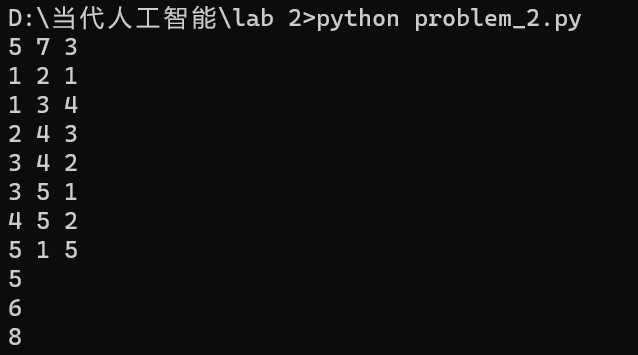
\includegraphics[width=0.5\linewidth]{image8.png}
    %\caption{Enter Caption}
    \label{fig:enter-label}
\end{figure}

\subsection{测试结果}
我们在Windows的命令行中,首先运行\lstinline|python problem_2.py|命令来启动程序,再把所有的输入内容复制黏贴在下面,再按一下回车键,就能得到算法的运行结果。将实验手册中的五个测试用例分别作为输入来运行上面的算法,结果如下图所示:
\begin{figure}[H]
    \centering
    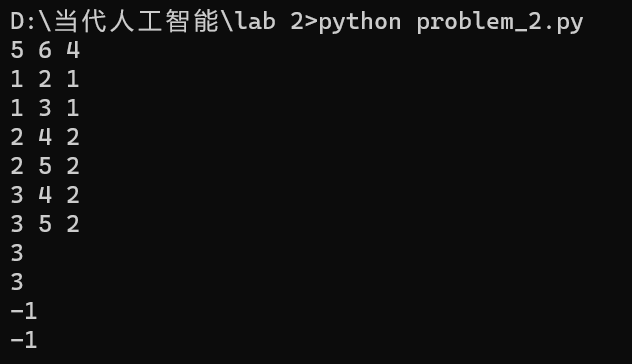
\includegraphics[width=0.5\linewidth]{image2.png}
    %\caption{Enter Caption}
    \label{fig:enter-label}
\end{figure}
\begin{figure}[H]
    \centering
    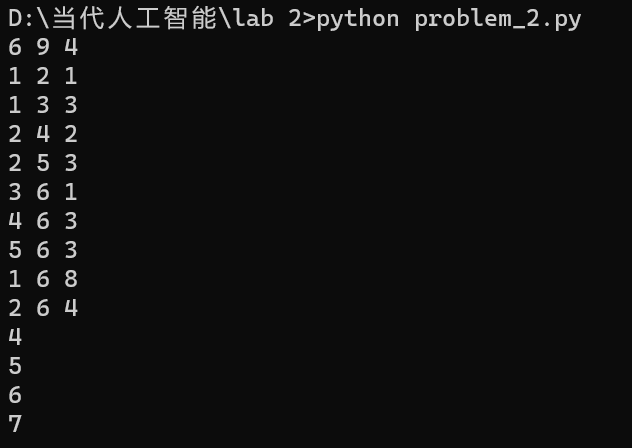
\includegraphics[width=0.5\linewidth]{image3.png}
    %\caption{Enter Caption}
    \label{fig:enter-label}
\end{figure}
\begin{figure}[H]
    \centering
    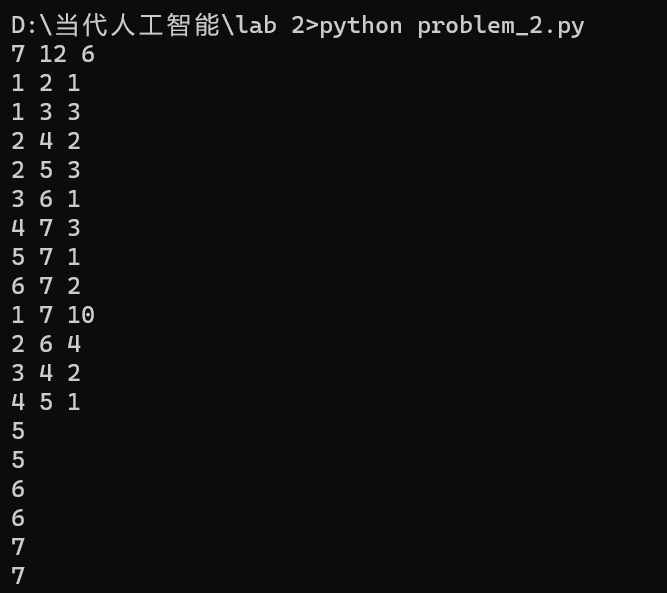
\includegraphics[width=0.5\linewidth]{image4.png}
    %\caption{Enter Caption}
    \label{fig:enter-label}
\end{figure}
\begin{figure}[H]
    \centering
    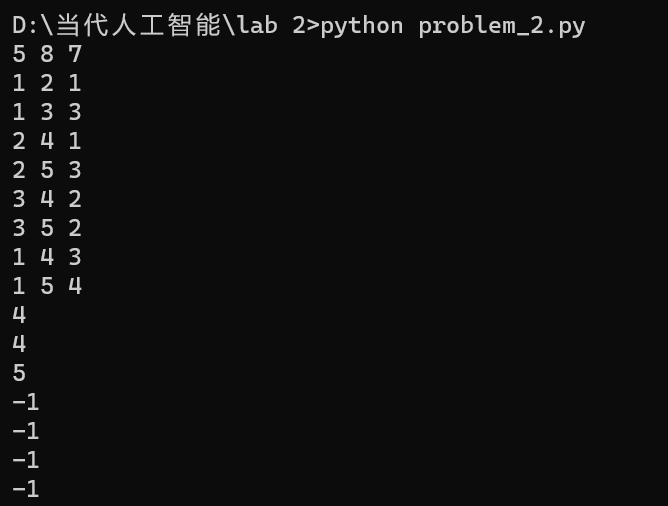
\includegraphics[width=0.5\linewidth]{image5.png}
    %\caption{Enter Caption}
    \label{fig:enter-label}
\end{figure}
\begin{figure}[H]
    \centering
    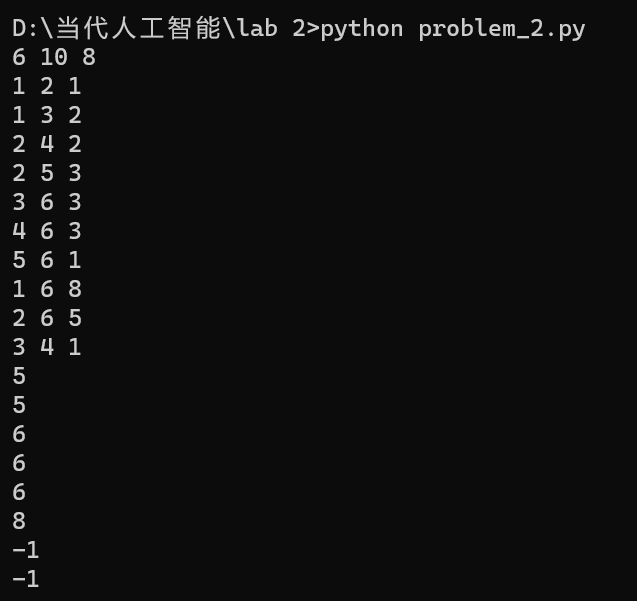
\includegraphics[width=0.5\linewidth]{image6.png}
    %\caption{Enter Caption}
    \label{fig:enter-label}
\end{figure}

\section{总结}
在本次实验中,我们用A*算法解决了两个搜索问题,体会到A*算法的强大之处:在启发式函数admissible(树搜索)或者具有consistency(图搜索)的前提下,A*算法能够很快地找到最优解。但是定义适合的启发式函数并不是特别简单的事。比如在问题二这样的路径搜索问题中,本应该是用某一点到目标节点的曼哈顿距离或欧氏距离来定义启发式函数的,但是在这个问题中我们并不知道节点之间的实际距离。在解决问题时,既要保证启发式函数能够在一定程度上反映节点之间的真实代价,又要保证启发式函数具备consistency,这让我纠结了很久,最终在反复理解了题意后才想出了现在的办法。但是在这种定义下,启发式函数的值过小,导致其在决定“哪个子节点要被弹出优先级队列”的时候起到的作用不大,在一定程度上失去了意义。所以说,如何根据实际的场景来定义启发式函数真的是一门学问。

\begin{thebibliography}{99}  

\bibitem{ref1}王万良:《人工智能导论》,高等教育出版社,2005年,第126页
\label{ref1}
\end{thebibliography}


\end{document}